%                      Code_Saturne version 1.3
%                      ------------------------
%
%     This file is part of the Code_Saturne Kernel, element of the
%     Code_Saturne CFD tool.
% 
%     Copyright (C) 1998-2007 EDF S.A., France
%
%     contact: saturne-support@edf.fr
% 
%     The Code_Saturne Kernel is free software; you can redistribute it
%     and/or modify it under the terms of the GNU General Public License
%     as published by the Free Software Foundation; either version 2 of
%     the License, or (at your option) any later version.
% 
%     The Code_Saturne Kernel is distributed in the hope that it will be
%     useful, but WITHOUT ANY WARRANTY; without even the implied warranty
%     of MERCHANTABILITY or FITNESS FOR A PARTICULAR PURPOSE.  See the
%     GNU General Public License for more details.
% 
%     You should have received a copy of the GNU General Public License
%     along with the Code_Saturne Kernel; if not, write to the
%     Free Software Foundation, Inc.,
%     51 Franklin St, Fifth Floor,
%     Boston, MA  02110-1301  USA
%
%-----------------------------------------------------------------------
%

\programme{condli}

\vspace{1cm}
%%%%%%%%%%%%%%%%%%%%%%%%%%%%%%%%%%
%%%%%%%%%%%%%%%%%%%%%%%%%%%%%%%%%%
\section{Fonction}
%%%%%%%%%%%%%%%%%%%%%%%%%%%%%%%%%%
%%%%%%%%%%%%%%%%%%%%%%%%%%%%%%%%%%
Il est n\'ecessaire de disposer de conditions aux limites dans au moins 
trois cas principaux~: 
\begin{itemize}
\item calcul de termes convectifs (diff\'erentiels d'ordre un en espace) au
bord~:  le calcul fait intervenir un flux au bord et demande 
la donn\'ee au bord de la variable convect\'ee lorsque la fronti\`ere est
``entrante'' au sens des courbes caract\'eristiques du syst\`eme 
(au sens de la vitesse, dans le cas d'une \'equation isol\'ee portant 
sur un simple scalaire~: interpr\'etation suffisante dans le cadre actuel de
\CS\footnote{sauf en module compressible, cf. \fort{cfxtcl}})~;
\item calcul de termes de diffusion (diff\'erentiels d'ordre deux en espace)~: 
il est alors n\'ecessaire de disposer d'un moyen de conna\^\i 
tre la valeur 
de d\'eriv\'ees spatiales d'ordre un au bord (plus exactement, il est
n\'ecessaire de disposer d'information permettant de calculer les termes qui en
d\'ependent, comme les contraintes ou les flux thermiques en paroi)~;
\item calcul de gradient ``cellules'' plus standard~: il est n\'ecessaire de disposer de la
donn\'ee de la variable aux faces de bord (plus g\'en\'eralement, il est n\'ecessaire
de disposer d'un moyen de calculer les termes discrets des \'equations 
lorsqu'ils font intervenir le gradient dans les cellules de bord, comme par
exemple les termes de gradient transpos\'e des \'equations de Navier-Stokes).
\end{itemize}

Les consid\'erations pr\'esentes concernent uniquement les variables de calcul 
(vitesse, pression, tenseur de Reynolds, scalaires solution d'une \'equation 
de convection-diffusion). Pour ces grandeurs\footnote{
Les autres grandeurs 
(propri\'et\'es physiques par
exemple) font l'objet d'un traitement diff\'erent qui ne sera pas d\'etaill\'e
ici (par exemple, pour la masse volumique, l'utilisateur d\'efinit directement 
les valeurs aux bord, information qui est conserv\'ee telle quelle~; on pourra 
se reportera \`a \fort{usphyv} ou \fort{phyvar}).
}, 
l'utilisateur doit d\'efinir
les conditions aux limites en chaque face de bord (\fort{usclim}). 
  

Le sous-programme \fort{condli} permet de traduire les donn\'ees utilisateur
(fournies dans \fort{usclim}) au format interne de repr\'esentation des conditions
aux limites. Des v\'erifications de compl\'etude et de coh\'erence sont
\'egalement men\'ees (dans \fort{vericl}). Sont en particulier trait\'ees les conditions aux limites
de paroi (\fort{clptur}) 
et de sym\'etrie pour les vitesses et le tenseur de Reynolds (\fort{clsyvt}). 

Le sous-programme \fort{condli} fournit en sortie des couples de coefficients 
$A_b$ et $B_b$ 
pour chaque variable~$f$ et chaque face  de bord. Ils sont utilis\'es pour le calcul des
termes discr\'etis\'es intervenant dans les \'equations \`a r\'esoudre et
permettent en particulier de d\'eterminer une valeur de face
de bord $f_{b,int}$ (localis\'ee au ``centre'' de la face de bord, 
barycentre de ses sommets) par la
relation $f_{b,int} = A_b+B_b\,f_{I'}$ o\`u $f_{I'}$ est la valeur de 
la variable au point
$I'$, projet\'e du centre de la cellule jouxtant le bord sur la droite 
normale \`a 
la face de bord et passant par son centre 
(voir la figure~\ref{Base_Condli_fig_flux_condli}). 

\begin{figure}[h]
\centerline{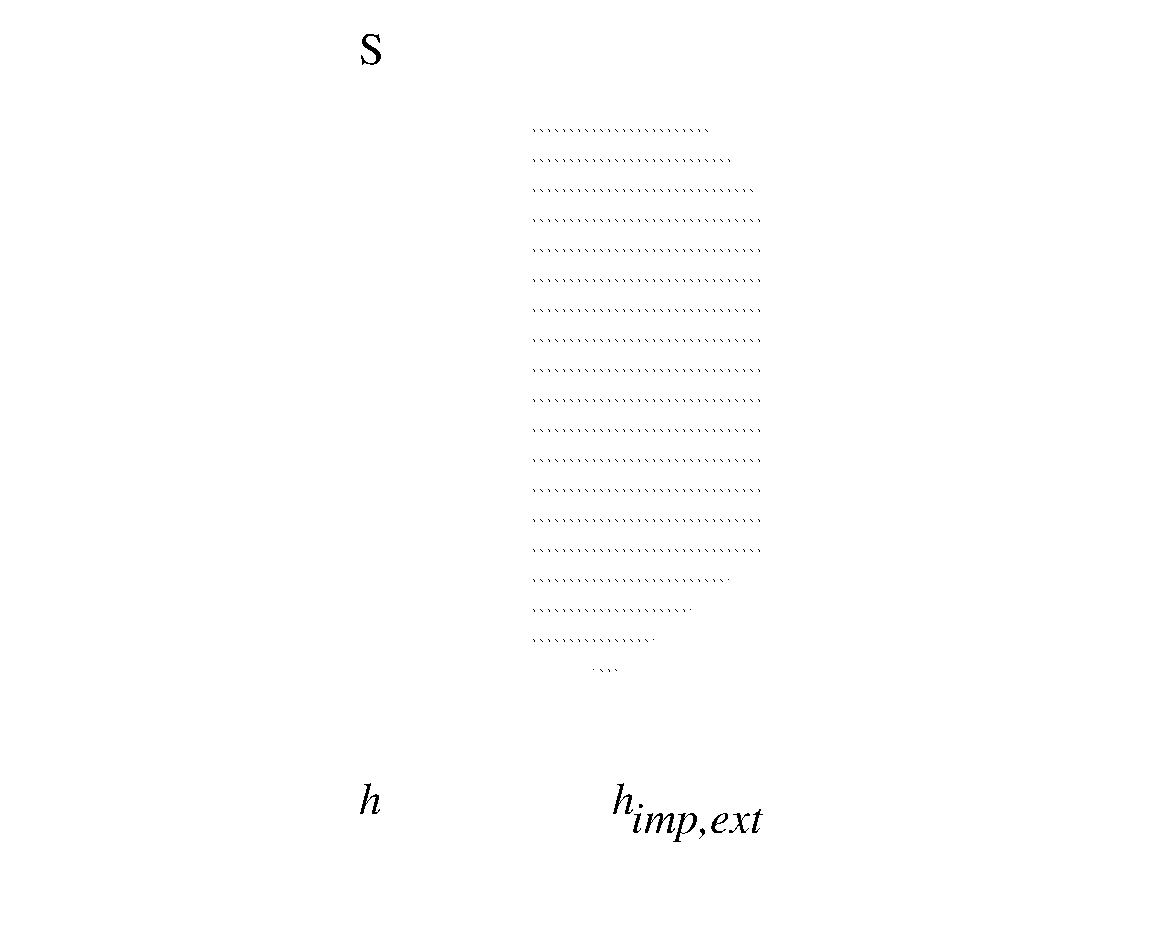
\includegraphics[height=8cm]{../Base/Condli/Images/fluxbord.pdf}}
\caption{\label{Base_Condli_fig_flux_condli}Cellule de bord.}
\end{figure}

